\section*{Aufgabe 2.1a) und 2.1b)}
In dieser Aufgabe war der gegebene Quelltext zu verwenden und so abzuändern, 
dass zwei Trajektorien mit beinahe gleichen Startbedingungen daraufhin
untersucht werden können, ab welchem Zeitpunkt die Differenz der Orte größer als
0,1 wird (siehe Aufgabenstellung). Diese Messung wird 200mal wiederholt, um
statistische Aussagen über diesen Zeitpunkt treffen zu können.

Der Octave-Quelltext dafür wird hier gezeigt:
\lstinputlisting[firstline=1,firstnumber=1,label=lst:chaos,caption={chaos.m}]{../chaos.m}

Wenn man diesen ausführt, so resultiert unter anderem der folgende Output:
\begin{lstlisting}[caption=Output unseres Programms,label=lst:output]
t_mean =  93.263
t_std =  26.290
t_conf_int =  1.8590
lamda_mean =  0.13447
lamda_std =  0.042518
\end{lstlisting}

Die auftretenden Werte sind:
\begin{itemize}
\item \texttt{t\_mean}: die mittlere Zeit, nach der die gewünschte Abweichung
  auftrat
\item \texttt{t\_std}: Standardabweichung von \texttt{t\_mean}
\item \texttt{t\_conf\_int}: Vertauensintervall von \texttt{t\_mean}
\item \texttt{lambda\_mean}: der Mittelwert der Variable λ, wie sie in der
  gegebenen Formel auftaucht
\item \texttt{lambda\_std}: Standardabweichung von λ
\end{itemize}

Wenn also die Startwerte der einen Trajektorie um etwa $10^{-6}$ von denen der
anderen abweichen, entwickelt sich im Mittel nach $93\pm2$ Zeiteinheiten eine
Differenz von 0,1 zwischen den Bahnen.

Wenn man die einzelnen Zeitpunkte histogrammiert, resultiert der folgende Plot
in \fref{hist_zeitschritte}.
\begin{figure}[htb]
  \centering
    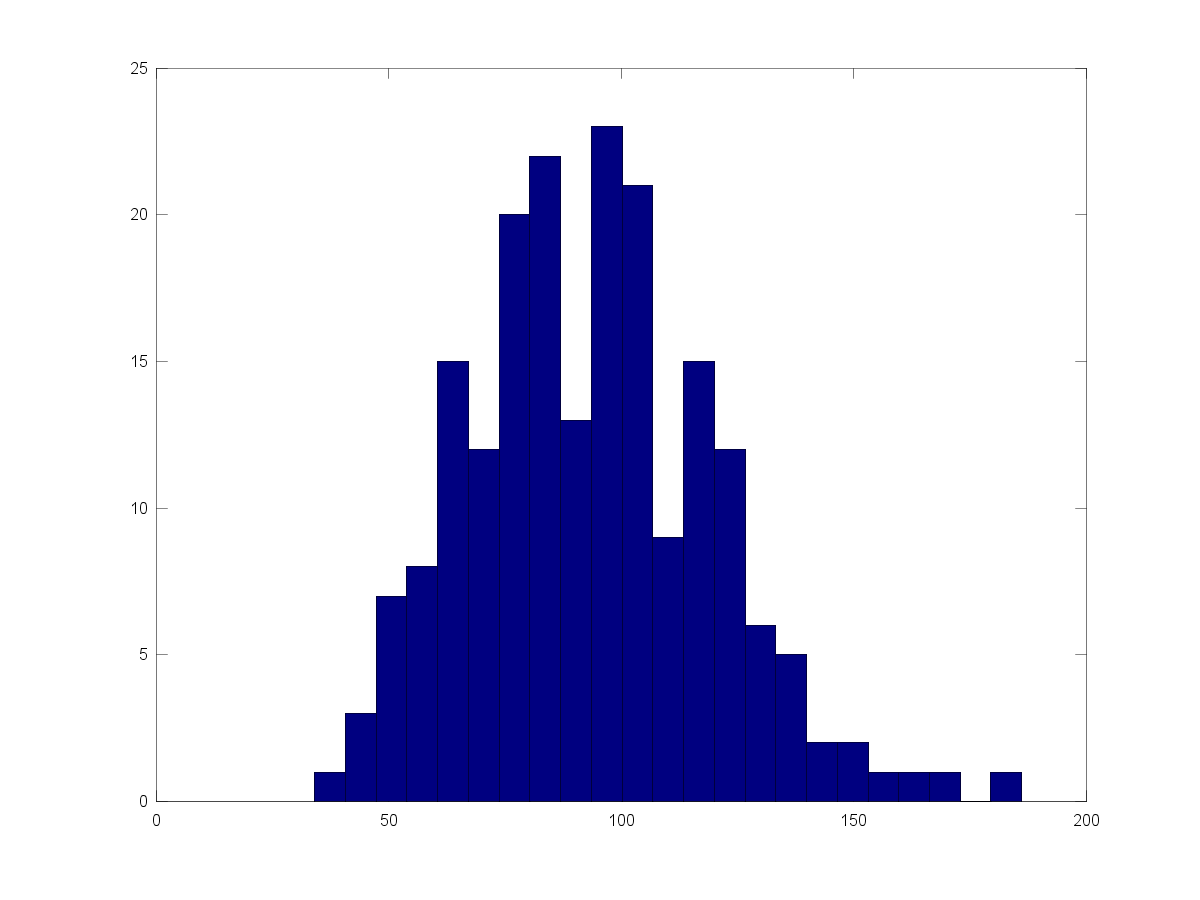
\includegraphics[width=1\columnwidth,keepaspectratio]{../figure_std}
    \caption{Statistik der Anzahl der benötigten Zeitschritte}
  \label{fig:hist_zeitschritte}
\end{figure}

